\chapter{Implementierung}
In diesem Kapitel wird zunächst die Implementierung der verschieden Ansätze in C++ behandelt. Hierbei wird auch auf die Besonderheiten des FPGA eingegangen. Des weiteren wird erläutert, wie der FPGA programmiert wird, vor allem in Hinblick auf die Parallelisierung der einzelnen Komponenten.
\section{Implementierung in C++}
Für die erste Implementierung der Voraussagefunktion wurde der Code von \cite{IMPL} aus Python in C++ übersetzt und an die Eigenschaften eines FPGA angepasst. In Abbildung 4.1 sind die Kernfunktionen des Programmcodes dargestellt. Die Funktion \textit{predict()} liefert die Berechnung der Formel $\dfrac{1}{1+\exp(-(\beta_0+x_i^T\beta))}$. Die Koeffizienten $\beta$ sind hier als Array $coefficients[\text{ }]$ gespeichert, zudem gibt es für die Batch-Realisierung ein Hilfsarray $tmp\textit{\_}coefficients[\text{ }]$. Der Datentyp \textit{DATA\_TYPE} kann hier zum einen Als Gleitkommazahl (\textit{float}), zu anderen als Fixkommazahl (\textit{ap\_fixed}) deklariert werden. Die Wahl für den Fixkomma-Datentyp fällt auf ein von Xilinx selbst bereitgestelltes Konstrukt \textit{ap\_fixed}, da es für das FPGA optimiert wurde und hier eine Vielzahl an Konfigurationen vorgenommen werden können. Die Gesamtanzahl der für eine Instanz belegten Bits wurde auf 16 festgelegt, davon ein Vorzeichenbit und 4 Vorkommastellen. Durch die Einstellung \textit{AP\_RND\_CONV} wird die Zahl, zum Beispiel nach einer Divisionsberechnung auf den nächsten repräsentierbaren Wert gerundet. Die Rundungsrichtung ist dabei abhängig von dem am wenigsten signifikanten Bit. Ist dieses gesetzt wird gegen $+\infty$, andernfalls gegen $-\infty$ gerundet.\cite{XIL2}
Um einem eventuellen Overflow der Zahl entgegenzuwirken wählt man die Einstellung \textit{AP\_SAT\_SYM}. Im Fall eines Positiven Overflows wird hierbei der höchste, bei einem negativen Overflow der kleinste darstellbare Wert gewählt.\cite{XIL2} Die FPGA Einstellung \textit{pragma HLS LOOP FLATTEN} sorgt für eine Parallelisierung der Schleife auf dem FPGA. Das funktioniert allerdings nur, wenn innerhalb der Schleife auf immer andere Ziele geschrieben wird. In der Funktion \textit{predict()} zum Beispiel wird die Variable \textit{yhat} immer wieder neu gesetzt, sodass eine Paralleliserung hier nicht möglich ist. 
\begin{figure}[ht]
\centering
\begin{lstlisting}
/* Voraussage treffen anhand logistischer Regression */
DATA_TYPE predict(){
    DATA_TYPE yhat = coefficients[0];
	for(int i=0; i<FEATURE_COUNT; i++){
		yhat+=coefficients[i+1]*features[i];
	}
	float tmp_yhat=-yhat;
	DATA_TYPE predicted=1.0f/(1.0f+hls::expf(tmp_yhat));
	return predicted;
}
\end{lstlisting}
\begin{lstlisting}
void learn(){
    DATA_TYPE predicted=predict();
    DATA_TYPE error=label-predicted;
    float sum_error_float=(float)sum_error+(float)error;
    sum_error=sum_error_float;
    tmp_coefficients[0]+=predicted*(1.0f-predicted);
	for(int i=0; i<FEATURE_COUNT; i++){
		#pragma HLS LOOP FLATTEN
		tmp_coefficients[i+1]+=predicted*(1.0f-predicted)*
			features[i];
	}
	/* Batch Update der Koeffizienten */
	batch_count++;
	if(batch_count>=BATCH_SIZE){
		DATA_TYPE sum_error_t=sum_error/BATCH_SIZE;
		for(int i=0; i<FEATURE_COUNT+1; i++){
			coefficients[i]+=lrate*sum_error_t*
				tmp_coefficients[i]/BATCH_SIZE;
		}
		batch_size=0;
	}
}
\end{lstlisting}
\caption{Codes des Perzeptrons}
\end{figure}
Die Funktion \textit{hls::expf()} wird von Xilinx geliefert und dient als Realisierung der Expotentialfunktion und ist für FPGAs optimiert.\\ 


Um die High-Performance Schnittstelle über PCIe von \cite{DILL} voll ausnutzen zu können wurde eine Trennung der Codeteile vorgenommen, damit ein Teil des Algorithmus auf dem FPGA und ein Teil auf dem Hostcomputer laufen kann. Der Hostrechner übernimmt hier die Vorbereitung der Daten und die Äußeren Schleifendurchläufe. Es werden immer die einzelnen Variablen mit dem dazugehörigen Label an den FPGA gesendet, welcher dann je nach Konfiguration damit trainiert oder eine Voraussage trifft. Der Vorteil hierbei ist, dass auf dem FPGA mehrere logistische Regressionen gleichzeitig implementiert sind, die mit verschiedenen Parametern (zum Beispiel einem C für die Fehlerbestrafungsgewichtung oder unterschiedlichen Lernraten) initialisiert wurden.\\
Um die Datenverteilung auf dem FPGA zu gewährleisten wurde sowohl eine Verteiler- als auch eine Sammlerklasse implementiert. Diese sind für dafür zuständig den Datenstrom von Daten und Konfigurationsparametern auf die jeweiligen Perceptrons zu verteilen beziehungsweise von diesen einzusammeln. Die Sammlerklasse markiert zusätzlich noch die ausgegebenen Daten mit der Identifikation des jeweiligen Perceptrons, damit die Ergebnisse nach einem Durchlauf zugeordnet werden können.
\section{Implementierung als Blockdesign}
Um Auf dem FPGA zu implementieren, muss der Code für den Verteiler, den Sammler und das Perceptron in eine IP (Intelectual Property) umgewandelt werden.
 \begin{figure}[ht]
\centering
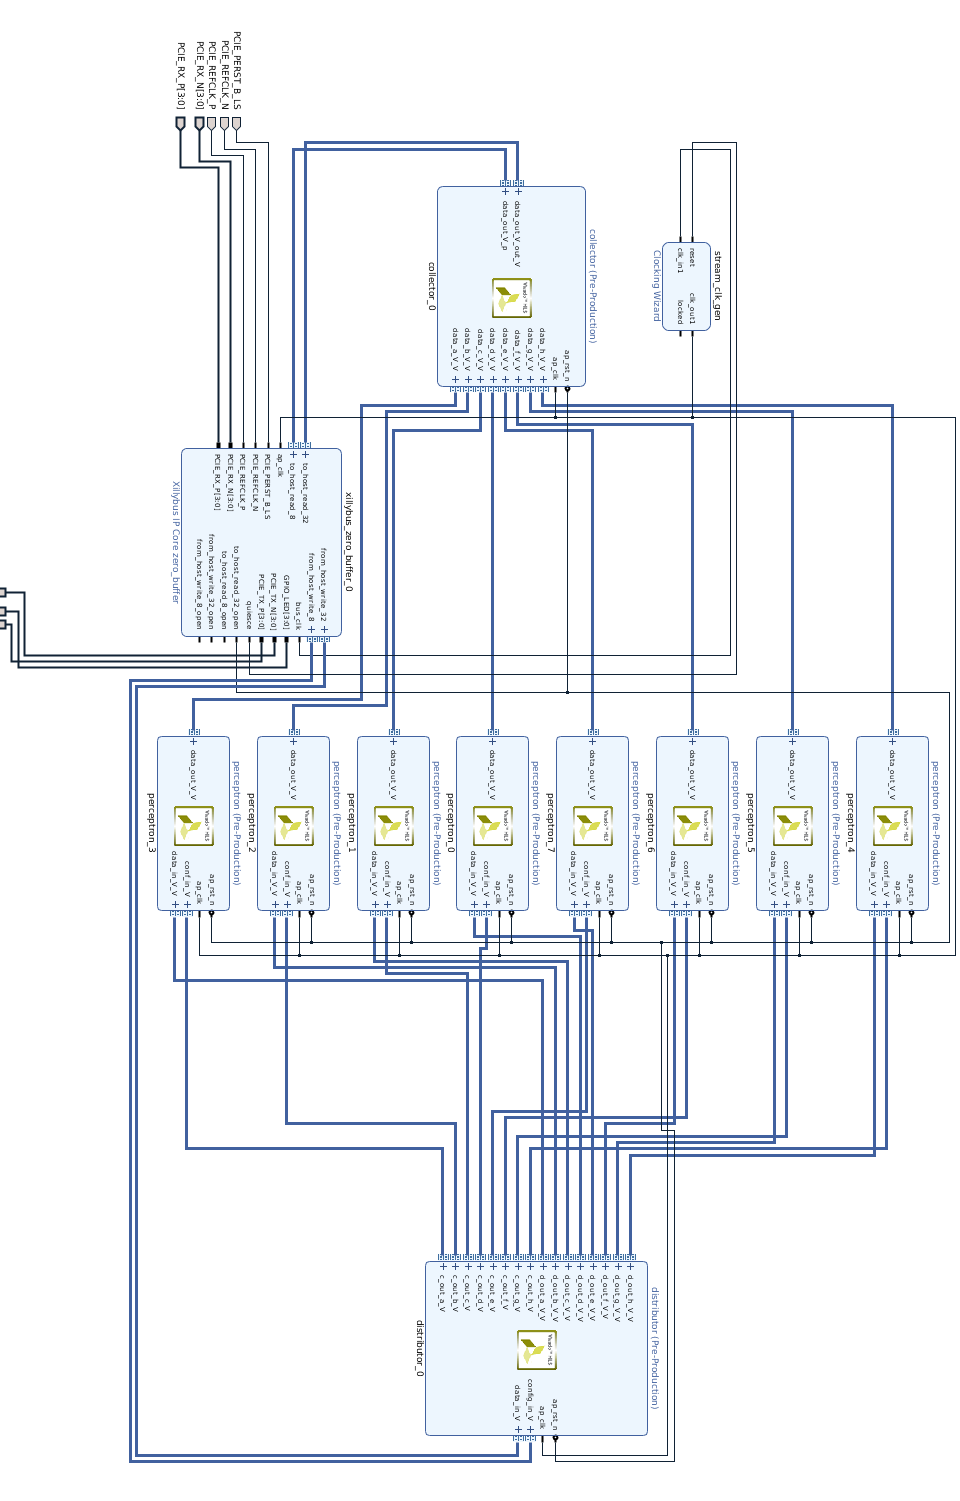
\includegraphics[scale=0.7]{bilder/blockdesign}
\caption{Das Blockdesign auf dem FPGA}
\end{figure}